\section{The Models}
\label{sec:models}

Real-time tracking applications often use
a Bayesian filtering approach,
or recursive Bayesian estimation,
in which the data is processed sequentially instead of all at once,
reducing computational demands
\citep{Anderson_2012}.
These models assume an underlying Markov process with state $\boldsymbol{\mathcal{X}}_k$,
an $n\times1$ column vector,
with system noise $\boldsymbol{\omega}_k\sim\mathrm{N}(\boldsymbol{0},\mathcal{Q})$ 
of which observations $\boldsymbol{\mathcal{Y}}_k$,
an $m\times1$ column vector, are made
with error $\boldsymbol{\nu}_k\sim\mathrm{N}(\boldsymbol{0},\mathcal{R})$,
giving the following general model:
\begin{equation}
\label{eq:rbe_model}
\begin{split}
\boldsymbol{\mathcal{X}}_k &= f(\boldsymbol{\mathcal{X}}_{k-1}, \boldsymbol{\omega}_k) \\
\boldsymbol{\mathcal{Y}}_k &= h(\boldsymbol{\mathcal{X}}_k) + \boldsymbol{\nu}_k
\end{split}
\end{equation}
The transition function $f:\mathbb{R}^n\mapsto\mathbb{R}^n$ 
describes the relationship between consecutive states,
while the measurement function $h:\mathbb{R}^n\mapsto\mathbb{R}^m$ is a deterministic function
mapping the underlying state to the observable state,
of which noisy measurements are made.



The following sections describe two Bayesian filters used in this application.
The first, implemented using a particle filter, estimates vehicle states
with the primary goal of estimating road travel times from a sequence of GPS positions.
The second uses these travel times to update road states 
and is implemented using an \emph{information filter},
a variant of the Kalman filter \citep{Anderson_2012}.



\subsection{Real-time vehicle model}
\label{sec:pf}

The underlying vehicle state at time $t_k$ consists of
the vehicle's distance travelled $x$ in meters along the route and
its speed $\dot x$ in meters per second.
These are combined into the state vector
$\bX_k = \left[x_k\ \dot x_k\right]^\top$,
of which observations $\bY_k$ are made using a GPS
with error $\omega^2$,
giving the longitude $\lambda_k$ and latitude $\phi_k$ of the vehicle
as $\bY_k = \left[\lambda_k\ \phi_k \right]^\top$.
We use a particle filter to estimate $\bX_k$
due to its flexibility and proven robustness
in recent vehicle modelling applications \citep{Ulmke_2006,Hans_2015}.
It also makes it trivial to estimate travel times
$\bz = (z_1,\ldots,z_L)^\top$, in seconds, along road segments
as the vehicle traverses the route.


The primary advantage of the particle filter is its handling of multimodality,
as demonstrated in Figure~\ref{fig:pf_state_predict},
which is a common feature of the proposal distribution, particularly around bus stops.
Another advantage is that the likelihood function is intuitive, based
on the physical distance between the vehicle observation and the state's
estimate of the actual location, $h(\bX_k)$ (Section~\ref{sec:pf_update}).
Conversely, particle filter methods are computationally demanding,
requiring an increasing number of particles as model complexity and
the number of parameters increases \citep{Carpenter_1999}.
Section~\ref{sec:rt} describes our implementation of the particle filter
and its \rt performance.

\begin{figure}[p]
    \centering
    \begin{subfigure}[t]{1\textwidth}
        \centering
        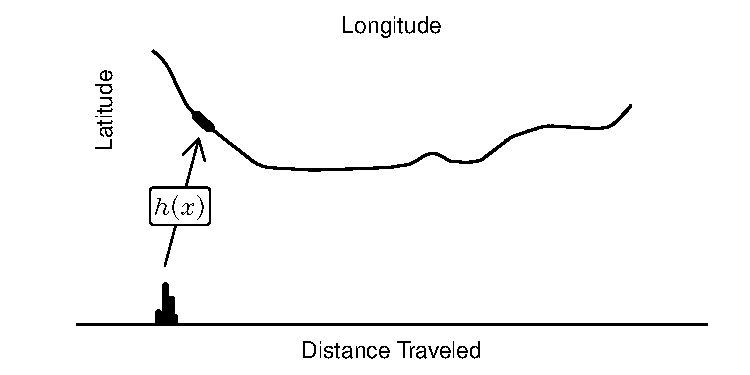
\includegraphics[width=0.7\textwidth]{figures/03_particle_filter_1.pdf}
        \caption{
            Vehicle state is mapped to observation space by the
            measurement function $h$.   
        }
        \label{fig:pf_state_prev}
    \end{subfigure}\\
    \begin{subfigure}[t]{0.9\textwidth}
        \centering
        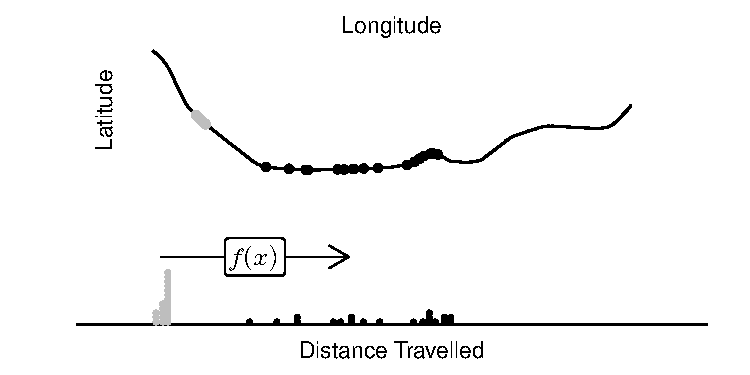
\includegraphics[width=0.7\textwidth]{figures/03_particle_filter_2.pdf}
        \caption{
            The transition function $f$ predicts the future state 
            of each particle.
        }
        \label{fig:pf_state_predict}
    \end{subfigure}\\
    \begin{subfigure}[t]{0.9\textwidth}
        \centering
        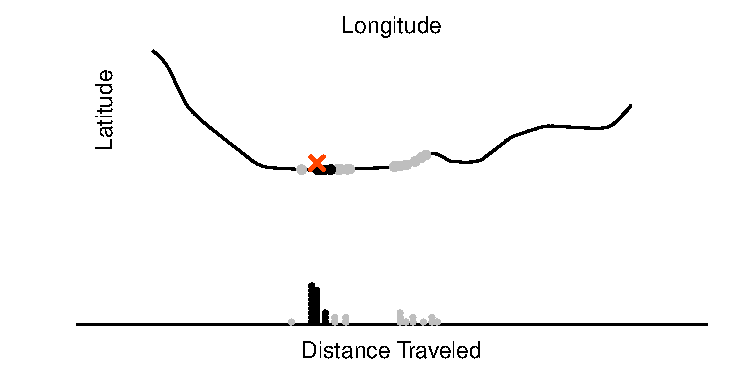
\includegraphics[width=0.7\textwidth]{figures/03_particle_filter_4.pdf}
        \caption{
            The state is updated by resampling with likelihood weights based on the distance
            between the particle and the observation, shown as a (red) cross.
        }
        \label{fig:pf_state_predict2}
    \end{subfigure}
    \caption{
        The particle filter approximates vehicle state using a set of 
        discrete points (a), which are each mutated independently (b)
        to predict the next state.
        The measurement function $h$ maps each particle state
        to a GPS coordinate (a),
        which can be compared to the observed location (c)
        to calculate each particle's likelihood to compute resampling weights.
    }
    \label{fig:pf_state}
\end{figure}

\afterpage{\clearpage}

In a particle filter, the posterior distribution of the state at time $t_{k-1}$
is represented by a set of discrete points, or particles, (Figure~\ref{fig:pf_state_prev}),
each with an associated weight $W_{k-1}^{(i)}$.
The state is expressed using the Dirac delta function $\dot\delta(\cdot)$,
so that
\begin{equation*}
p(\bX_{k-1} | \bY_{1:k-1}) \approx 
    \sum_{i=1}^N W_{k-1}^{(i)} \dot\delta(\bX_{k-1} - \bX_{k-1}^{(i)})
\end{equation*}
each of which is independently updated or \emph{mutated} using the transition function $f$ (Figure~\ref{fig:pf_state_predict}),
\begin{equation*}
p(\bX_k | \bX_{k-1}) \approx 
    \sum_{i=1}^N W_{k-1}^{(i)} \dot\delta(\bX_{k} - f(\bX_{k-1}^{(i)}, \boldsymbol{\psi})),
\end{equation*}
where $\boldsymbol{\psi}$ is a vector containing all of the necessary model parameters
(Section~\ref{sec:pf_prediction}).
After mutation, 
the state is updated by reweighting the particles using the likelihood $p(\bY_k | \bX_k^{(i)})$ 
(Section~\ref{sec:pf_update}) and standardising so $\sum_{i=1}^N W_k^{(i)} = 1$,
\begin{equation*}
W_k^{(i)} = \frac{W_{k-1}^{(i)} p(\bY_k | \bX_k^{(i)})}{
    \sum_{j=1}^N W_{k-1}^{(j)} p(\bY_k | \bX_k^{(j)})
}
\end{equation*}
which gives us the final posterior state estimate
\begin{equation*}
p(\bX_k | \bY_k) \approx  
    \sum_{i=1}^N W_{k}^{(i)} \dot\delta(\bX_{k} - \bX_{k}^{(i)}).
\end{equation*}

One problem with particle filters is degeneration:
when the particles become too spread out with respect to the predictive distribution,
the weight will be concentrated on to just a few of them.
This occurs naturally over time, but the rate at which it does so depends 
on a relationship between how well the transition function predicts future states
and the variance of those predictions (system noise).
To avoid degeneration,
particle filters use \emph{importance resampling}
using importance weights $\{W_k^{(1)}, \ldots, W_k^{(N)}\}$,
thereby removing improbable particles and replacing them with more probable ones,
as demonstrated in Figure~\ref{fig:pf_state_predict2}.
However, resampling requires sorting $N$ particles,
which is of $\mathcal{O}(N\log N)$ complexity,
so to reduce computational costs, resampling is performed only when
the effective sample size $N_{\text{eff}} = 1 / \sum_i (W_k^{(i)})^2$
falls below a specified threshold $N_{\text{thres}}$
\citep{Gustafsson_2002}.
We used a fixed threshold value of $N_{\text{thres}} = N/4$
for the current work.


\subsubsection{Vehicle transition function}
\label{sec:pf_prediction}

The particle filter allows us to flexibly model bus behaviour,
which currently includes
\begin{enumerate}
\item non-constant speed along roads (between observations), and
\item bus stop behaviour, which involves optional stopping and waiting times
    while passengers board and disembark.
\end{enumerate}
The transition function consists of two models,
one for each of the above behaviours.
The first models the speed and distance travelled by the vehicle,
\begin{equation}
\label{eq:trans_newton}
\bX_k^{(i)} = f(\bX_{k-1}^{(i)}, \delta_k, \epsilon_k^{(i)}) = 
    \begin{bmatrix}
        x_{k-1}^{(i)} + \delta_k(\dot x_{k-1}^{(i)} + \epsilon_k^{(i)}) \\
        \dot x_{k-1}^{(i)} + \epsilon_k^{(i)}
    \end{bmatrix},
\end{equation}
where $\delta_k = t_k - t_{k-1}$
and $\epsilon_k^{(i)}\sim\mathrm{N}_T(0, \sigma^2)$, truncated to the interval
$(-\dot x_{k-1}^{(i)}, 30 - \dot x_{k-1}^{(i)})$
to ensure vehicle speed is always positive and less than 30~m/s
(approximately 110~km/h).


The second vehicle behaviour requires a model of bus stop wait times.
When the vehicle is approaching stop $j$,
it stops with some probability $\pi_j$.
If it does not stop, the remaining travel time $\delta_k$ is unaltered;
otherwise, the bus waits for a minimum of $\gamma$ seconds---this 
accounts for deceleration, opening and closing of doors, and acceleration
\citep{Hans_2015}---and then waits while passengers board and disembark,
which is assumed to be exponentially distributed with mean $\tau_j$.
This behaviour is expressed in the following model:
\begin{equation}
\label{eq:trans_stop}
\begin{split}
p_j^{(i)} &\sim \mathrm{Bernoulli}(\pi_j) \\
\tilde d_j^{(i)} &\sim \mathrm{Exponential}(\tau_j) \\
d_j^{(i)} &= p_j^{(i)}(\gamma + \tilde d_j^{(i)}).
\end{split}
\end{equation}


The model components are implemented as an algorithm,
in which (\ref{eq:trans_newton}) is evaluated iteratively one second at a time,
decreasing $\delta_k^{(i)}$ by one each time,
after initializing $\delta_k^{(i)} = \delta_k$.
In order to obtain the desired non-constant speed between observations,
$\epsilon_k^{(i)}$ is re-sampled each second,
allowing the particle's speed to vary.
This iterative approach allows the particle to approach the next stop,
at which point (\ref{eq:trans_stop}) is evaluated for the particle
and the dwell time subtracted from $\delta_k^{(i)}$.
This process continues until $\delta_k^{(i)}$ reaches zero.
The algorithm also keeps track of each particle's travel time $z_\ell^{(i)}$
along each segment $\ell$ of the route,
storing the times so that the posterior distribution of the travel time
can be computed once all particles have completed segment $\ell$:
\begin{equation}
\label{eq:post_tt}
p(z_\ell | \bY_{1:k}) \approx
    \sum_{i=1}^N W_k^{(i)} \dot\delta(z_\ell - z_\ell^{(i)}).
\end{equation}



\subsubsection{Updating state using the observation likelihood}
\label{sec:pf_update}

Computing the likelihood of the observation given each particle state,
$p(\bY_k|\bX_k^{(i)})$,
uses the measurement function $h$ and 
a \emph{geographical projection} function $g$ to allow comparison of $\bY_k$,
a GPS observation, with $\bX_k$, a distance travelled along the route in meters.

The measurement function $h$ computes GPS coordinates by using the 
shape information provided by GTFS and travelling $x_k$ meters along 
this two-dimensional line.
Meanwhile, we use the \emph{Equirectangular projection} \citep{Snyder_1998},
$\br = g(\bY_1 | \bY_0)$,
such that the magnitude of $\boldsymbol{r}$ is equal to the physical distance
between $\bY_0$ and $\bY_1$ and both dimensions are in meters.
Let $\bY_i = [\lambda_i, \psi_i]^\top$,
with $\lambda_i$ and $\psi_i$ measured in radians,  
and $R$ is the Earth's radius, in meters, then
\begin{equation}
\br = 
g(\bY_1 | \bY_0) = 
    \begin{bmatrix}
        r_1 \\ r_2
    \end{bmatrix} =
    R \begin{bmatrix}
        (\lambda_1 - \lambda_0)\cos\phi_0 \\
        \phi_1 - \phi_0
    \end{bmatrix}
\end{equation}
and, more importantly, the geographical distance $\mathcal{D}$ between the two 
GPS coordinates is given by
\begin{equation}
\label{eq:dist}
\mathcal{D}(\bY_0, \bY_1) = ||g(\bY_0 | \bY_1)|| = \sqrt{r_1^2 + r_2^2}.
\end{equation}


Now we assume GPS observations have a known error of $\omega^2$ meters,
and that \mbox{$\br \sim \mathrm{N}(\boldsymbol{0}, \omega^2\mathbf{I})$},
which allows us to express $\br$ in terms of two independent
standard normal random variables $z_1, z_2 \sim \mathrm{N}(0,1)$.
Now the distance between a vehicle observation $\bY_k$
and a state $\bX_k$, using (\ref{eq:dist}) and the measurement function $h$,
is expressed as
\begin{equation}
\label{eq:obs_dist}
\mathcal{D}(\bY_k, h(\bX_k)) = \sqrt{r_{k1}^2 + r_{k2}^2} 
    = \sqrt{(\omega z_1)^2 + (\omega z_2)^2}
    = \sqrt{\omega^2 (z_1^2 + z_2^2)}.
\end{equation}

Finally, the sum of two independent 
standard normal random variables has a Chi-square distribution with two degrees of freedom,
which is also an exponential distribution with rate~$\frac{1}{2}$,
and if $Z \sim \mathrm{Exponential}(\theta)$ then
$cZ \sim \mathrm{Exponential}(\frac{\theta}{c})$;
therefore, the \emph{squared} distance from (\ref{eq:obs_dist}) is distributed as
\begin{equation}
\label{eq:obs_exp}
\mathcal{D}(\bY_k, h(\bX_k))^2 =
\omega^2(z_1^2 + z_2^2) \sim \mathrm{Exponential}\left(\frac{1}{2\omega^2}\right).
\end{equation}

The likelihood of the observation $\bY_k$ given a state estimate $\bX_k^{(i)}$
can now be expressed using (\ref{eq:obs_exp}) 
and the probability density function of the exponential distribution,
\begin{equation}
\label{eq:lhood}
p(\bY_k | \bX_k^{(i)}, \omega) =
\frac{1}{2\omega^2}\exp\left\{
    -\frac{\mathcal{D}(\bY_k, h(\bX_k^{(i)}))^2}{2\omega^2}
\right\},
\end{equation}
where the distance between two GPS coordinates is easily computed,
allowing for fast evaluation of (\ref{eq:lhood}) within the particle filter algorithm.


It is worth noting that this representation of the likelihood is only
possible due to the discrete nature of the particle filter state estimate;
the Kalman filter---which has often been used for transit vehicle tracking---%
uses the measurement \emph{matrix}, requiring a linear
transformation between the state and its observations.
To do so, applications first estimate the \emph{observed distance travelled}
by snapping the GPS observations to the route,
which introduces unnecessary error and uncertainty into the model.
Our approach avoids this, which makes it more stable in locations where two 
parts of the route are close to each other,
such as at loops, where a single GPS observation might have two likely ``snapping'' points.


\subsection{Network model}
\label{sec:kf}

The primary objective of the network model is to estimate the \rt traffic conditions
(travel time) along roads in the transit network
and make short-term forecasts for estimating arrival times.
In this paper, we model each road segment independently,
as excluding correlations not only simplifies the model to a one-dimensional Kalman filter,
but it also means computations can be run in parallel,
further improving the real-time performance of the model.


The network state $\boldsymbol\theta_c = \{\theta_c^\ell\}_{\ell = 1}^L$ is the travel time 
of transit vehicles along road segment $\ell$ at time $t_c$,
of which observations $Z_{c\ell}^{m}$
are obtained from the particle filter for vehicle $m$ at time $t_c$,
as defined in (\ref{eq:post_tt}), such that 
(after adding the $m$ superscript to identify unique vehicles), 
\begin{equation}
\label{eq:tt_obs_mean}
Z_{c\ell}^{m} = \mathrm{E}(z_{\ell}^{m} | \bY^m_{1:c}) = 
\sum_{i=1}^N (W_c^{(i)})^m (z_\ell^{(i)})^{m}.
\end{equation}
The measurement error is also estimated from the particle filter,
\begin{equation}
\label{eq:tt_obs_err}
R_{c\ell}^m = \mathrm{Var}(z_{\ell}^{m} | \bY^m_{1:c}) = 
\sum_{i=1}^N (W_c^{(i)})^m \left((z_\ell^{(i)})^{m} - Z_{c\ell}^{m}\right)^2.
\end{equation}

The model of travel times becomes a simple reduction of (\ref{eq:rbe_model}) 
to the one-dimensional case, 
with $f$ and $h$ both unity,
system noise $v_{c\ell} \sim \mathrm{N}(0, \nu_\ell^2)$,
where $\nu_\ell^2$ is the average change in travel time per second
along road segment $\ell$,
the observation error $e_{c\ell}^{m} \sim \mathrm{N}(0, R_{c\ell}^{m})$,
and $\Delta_c = t_c - t_{c-1}$
\begin{equation*}
\begin{split}
\theta_c^\ell &= \theta_{c-1}^\ell + \Delta_{c\ell} v_{c\ell} \\
Z_{c\ell}^{m} &= \theta_c^\ell + e_{c\ell}^{m}
\end{split}
\end{equation*}


Since multiple vehicles can travel along a road simultaneously,
we used an information filter to implement the network model.
The information filter is a transformation of the Kalman filter in which the
\emph{information matrix} and \emph{information vector} are used in place of 
the covariance matrix and state vector, respectively,
allowing multiple observations to be added together to update the state
in a single iteration.


The state at time $t_{c-1}$ is parameterised by its mean and variance,
conditional on $\boldsymbol{Z}_{1:c-1,\ell}$, 
the data from all vehicles up until time $t_{c-1}$,
\begin{equation*}
\hat \theta_{c-1|c-1}^\ell = 
\mathrm{E}(\theta_{c-1}^\ell | \boldsymbol{Z}_{1:c-1,\ell})
\quad\text{and}\quad
P_{c-1|c-1}^\ell = 
\mathrm{Var}(\theta_{c-1}^\ell | \boldsymbol{Z}_{1:c-1,\ell})
\end{equation*}
respectively,
which are predicted from the previous state estimate using the predictive model
\begin{align*}
\label{eq:kf_transition}
\hat \theta^\ell_{c|c-1} &= \hat \theta^\ell_{c-1|c-1} \\
P^\ell_{c|c-1} &= P^\ell_{c-1|c-1} + (\Delta_{c\ell} \nu_{c\ell})^2
\end{align*}

For the update step, the parameters are transformed into an information
space parameterised by the information matrix $U^\ell_c = (P_{c|c-1}^\ell)^{-1}$
and the information vector $u^\ell_c~=~\hat \theta^\ell_{c|c-1} (P^\ell_{c|c-1})^{-1}$.
The travel time estimate of vehicle $m$ along segment $\ell$,
along with its uncertainty, 
as defined in (\ref{eq:tt_obs_mean}) and (\ref{eq:tt_obs_err}), respectively,
are transformed to a measurement information covariance matrix 
$B_{c\ell}^{m}~=~(R_{c\ell}^m)^{-2}$
and measurement information vector $b_{c\ell}^{m}~=~Z_{c\ell}^{m} (R_{c\ell}^{m})^{-2}$.
The total information is the sum of the information over all $M_{c\ell}$ vehicles
that traversed segment $\ell$ in the time interval $(t_{c-1}, t_c]$,
so the update equation is
\begin{align*}
U^\ell_{c|c} &= U^\ell_{c|c-1} + \sum_{m=1}^{M_{c\ell}} B_{c\ell}^{m} \\
\hat u^\ell_{c|c} &= \hat u^\ell_{c|c-1} + \sum_{m=1}^{M_{c\ell}} b_{c\ell}^{m}.
\end{align*}
The desired parameter estimates are obtained 
by the inverse transformations
\begin{equation*}
\hat \theta^\ell_{c|c} = \frac{\hat u^\ell_{c|c}}{U^\ell_{c|c}} 
\quad\text{and}\quad
P^\ell_{c|c} = \frac{1}{U^\ell_{c|c}}
\end{equation*}
which can now be used in the prediction of travel times
for upcoming buses. 
Note that, if we included segment correlations,
the full state $\boldsymbol{\theta}_c$ would need updating in a single step,
which would require inverting a large $L\times L$ matrix,
significantly increasing the time of updating the state.



